%%%%%%%%%%%%%%%%%%%%%%%%%%%%%%%%%%%%%%%%%%%%%%%%%%%%%%%%%%%%%%%%%
%_____________ ___    _____  __      __ 
%\____    /   |   \  /  _  \/  \    /  \  Institute of Applied
%  /     /    ~    \/  /_\  \   \/\/   /  Psychology
% /     /\    Y    /    |    \        /   Zuercher Hochschule 
%/_______ \___|_  /\____|__  /\__/\  /    fuer Angewandte Wissen.
%        \/     \/         \/      \/                           
%%%%%%%%%%%%%%%%%%%%%%%%%%%%%%%%%%%%%%%%%%%%%%%%%%%%%%%%%%%%%%%%%
%
% Project     : Seminararbeit
% Title       : 
% File        : einfluss.tex Rev. 00
% Date        : 10.10.2012
% Author      : Till J. Ernst
%
%%%%%%%%%%%%%%%%%%%%%%%%%%%%%%%%%%%%%%%%%%%%%%%%%%%%%%%%%%%%%%%%%
\thispagestyle{empty}
\chapter{Einfluss \textit{Sozialer Medien} auf das \textit{Subjektive Wohlbefinden}}\label{chap.einfluss}
\glsreset{swb}
In diesem Kapitel wird der Einfluss erläutert, wie sich \gls{sm} auf das \gls{swb} auswirken. Dazu werden verschieden Studien untersucht und mittels \gls{cm} grafisch zusammengeführt. Der Einfluss auf das \gls{swb} ist von verschiedenen Faktoren abhängig, welche in \textit{Abbildung~\ref{fig.ConceptMapSwbSm}} ersichtlich sind.\newline
Die Grafik stellt den Zusammenzug unterschiedlicher Studien dar, die sich mit den Auswirkungen von \gls{sm} auf das \gls{swb} auseinander setzen. Darin sind die verschiedenen Konstrukte ersichtlich, die in den Studien verwendet wurden. Gelesen wird die Grafik ausgehend von den \gls{sm} entlang den Verbindungslinien bis hin zum \gls{swb}.\newline
Innerhalb der Grafik wurden die Englischen Begriffe aus den Studien übernommen. Bei den Verbindungslinien wurde mit Deutschen Wörtern gearbeitet.\newline
In den folgenden Unterkapiteln werden diese Konzepte anhand der Grafik erläutert. Dazu wird die Grafik in verschiedene Stränge unterteilt, um den komplexen Informationsgehalt in übersichtliche Häppchen aufzuteilen. Die Stränge sollen von den \gls{sm} ausgehend, über wichtige Konzepte und Begriffe, bis hin zum \gls{swb} führen. Da es sich um eine komplexe Thematik handelt, ist es nicht immer möglich die Grenzen scharf zu ziehen. Viele Konzepte überschneiden sich und greifen ineinander über.\newline
Die in den folgenden Kapitel werden die in der Grafik markierten Begriffe näher erläutert. Wo dies möglich ist, werden die Englischen Begriffe in die entsprechend Deutschen Begriffe übersetzt. Für Begriffe, bei denen die ursprüngliche Bedeutung durch einen unsachgemässe Übersetzung gefährdet ist, oder das Deutsche Pendant dazu fehlt, wird das Originale Englische Wort übernommen. Zusätzlich wird bei den jeweiligen Worterklärungen dem Englischen Begriff eine mögliche Deutsche Übersetzung mitgeliefert, wobei hier zu beachten ist, dass die Begriffe in den Studien nicht immer identisch verwendet werden und die Bedeutung je nach Verwendung des Autors leicht abweichen kann.\newline 

%Abbildung von ConceptMap SWB und SM
\begin{figure}[H]
	\centering
		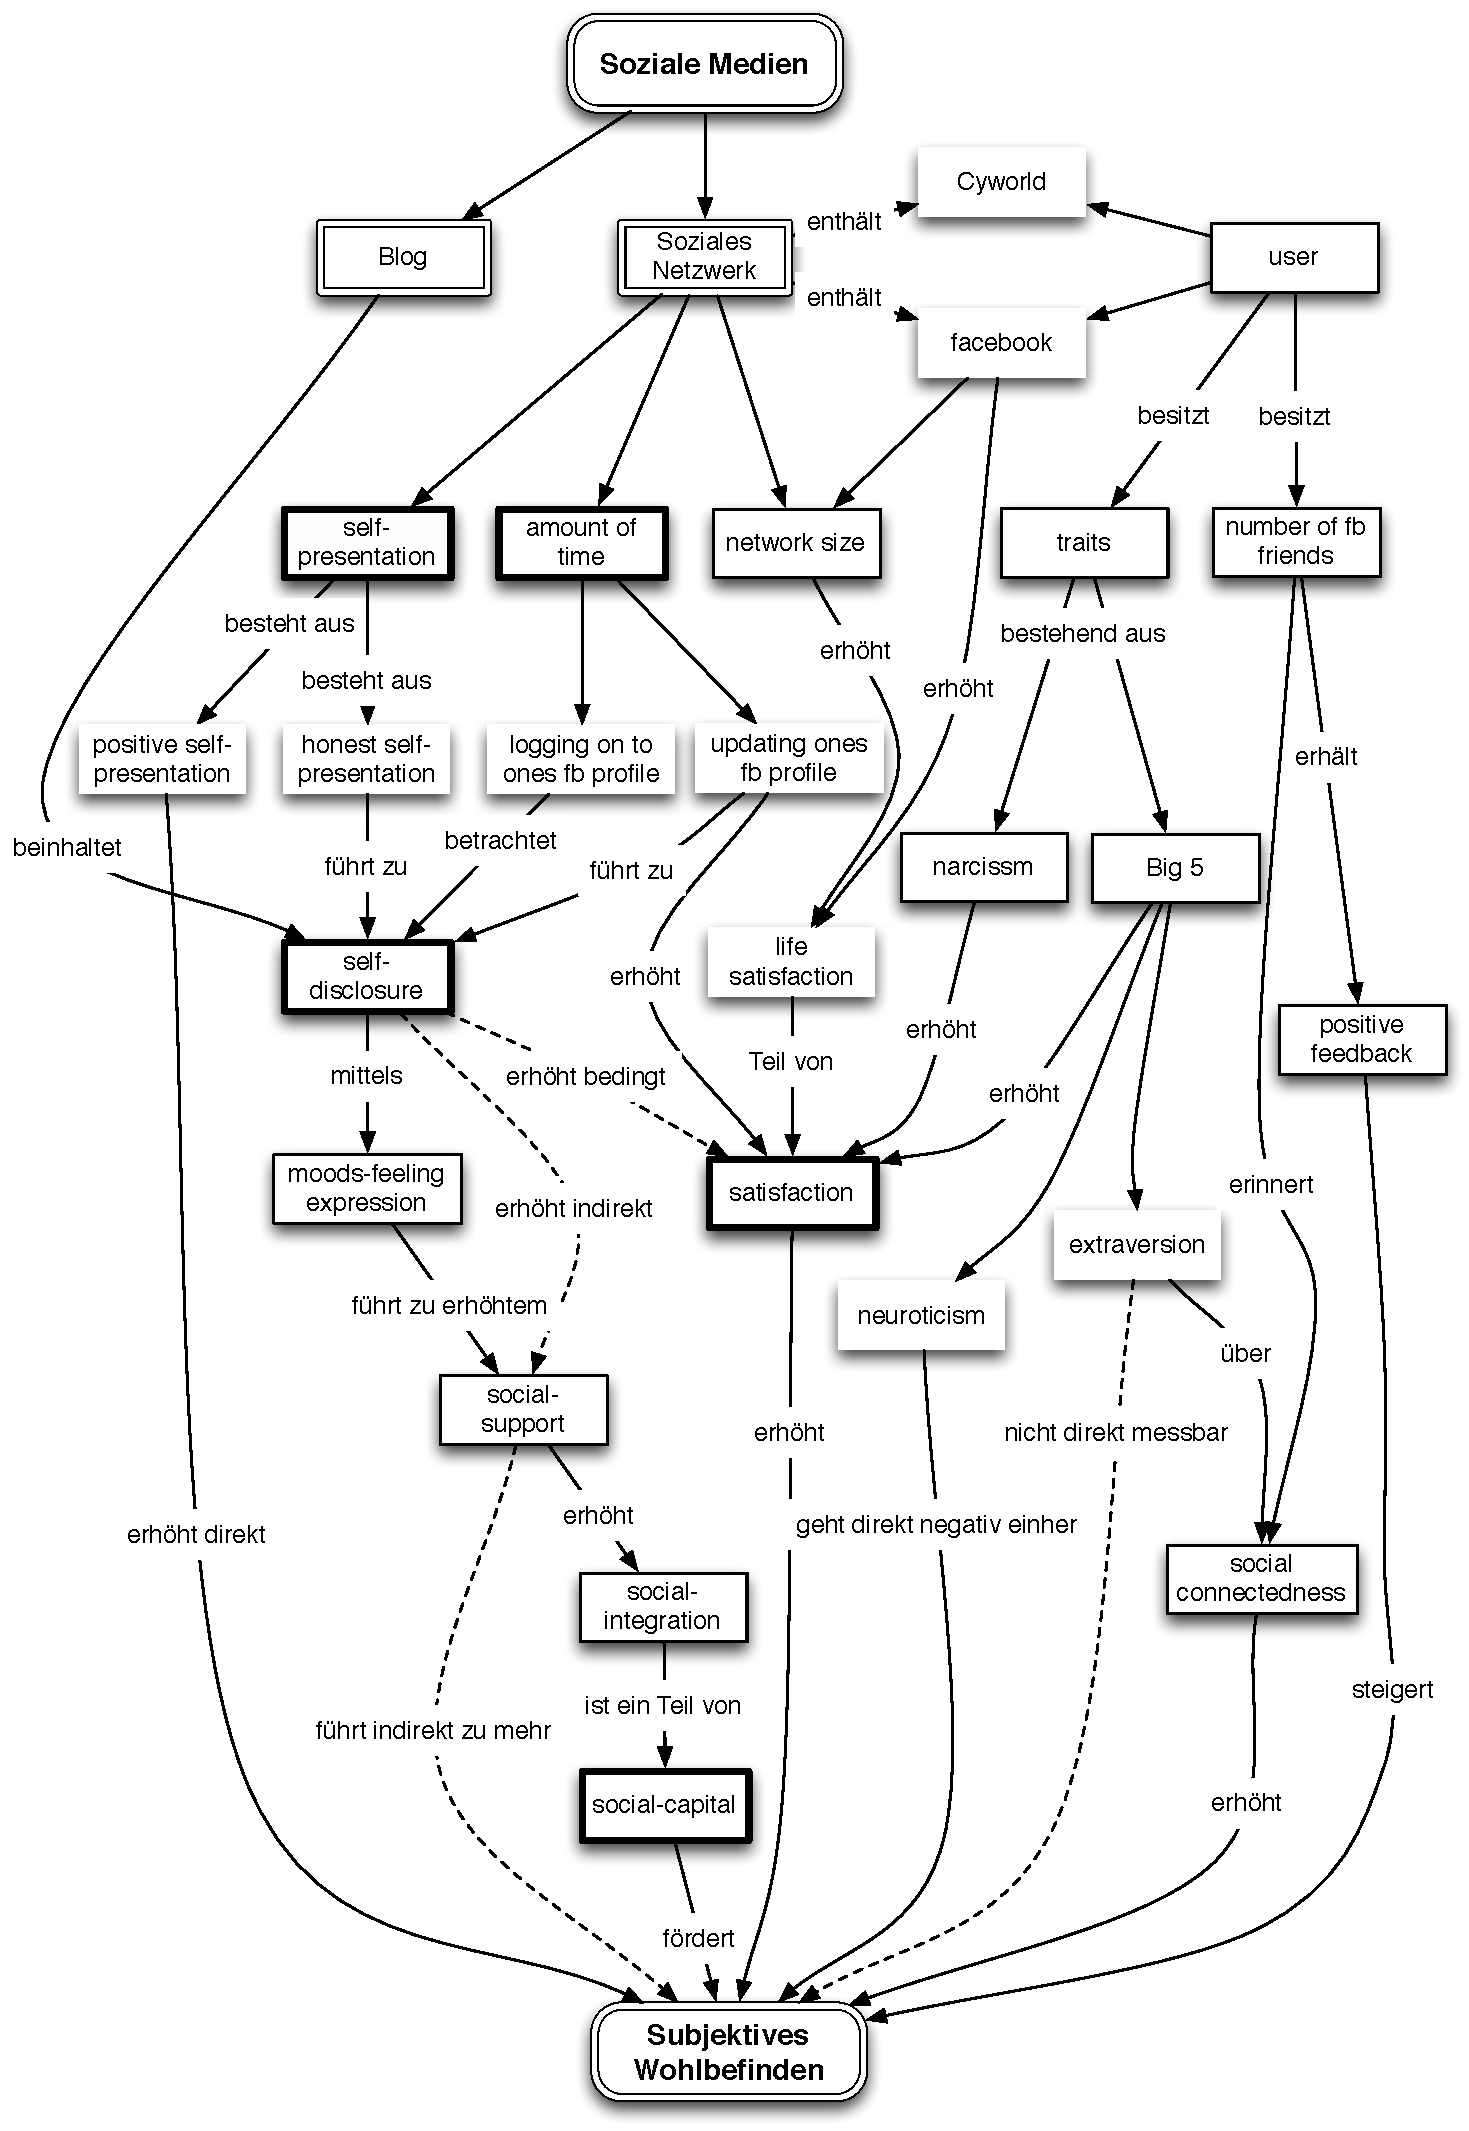
\includegraphics[width=0.8\textwidth]{images/grafiken/conceptMap_Swb_Sm_v2.pdf}
	\caption{ConceptMap - Subjektives Wohlbefinden und Soziale Medien}
	\label{fig.ConceptMapSwbSm}
\end{figure}

%UK Self-Presentation, Self-dicslosure und social capital
%----------------------------------------------------------------------
\section{\textit{Self-presentation}, \textit{self-disclosure} und \textit{social capital}}\label{sub.selfp}
In diesem Kapitel wird auf den Einfluss von \textit{self-presentation} und \textit{self-disclosure}, als Haupteinflussgrössen auf das \textit{\gls{swb}} eingegangen. \newline
%SubSec Einführung
\subsection{Einführung}\label{subsec.selfpEinführung}
Unter \textbf{self-presentation} (\textit{dt. Selbstdarstellung}) wird eine Strategie verstanden, die im Kontext von \textit{Facebook} näher untersucht wurde \cite[S.359ff]{Kim:2011}. \textit{Facebook} stellt nicht nur Mechanismen zur Verfügung, um Benutzerverbindungen untereinander grafisch darzustellen, sondern auch technologische Möglichkeiten wie sich Benutzer selber darstellen können \cite{Ellison:2007.1}. Je nach dem welche Möglichkeiten ein Benutzer verwendet (z.B.: Statusaktualisierung, erstellen und pflegen eines Fotoalbums, Nachrichten auf dem eigenen Profil posten, etc.) stellen sich diese Benutzer unterschiedlich getreu dar. In der Literatur wird innerhalb der \textit{\gls{cmc} (dt. Computervermittelte Kommunikation)} \cite{Tidwell:2002} und \textit{self-presentation} auf online Partnervermittlungsplattformen \cite{Gibbs:2006} zwischen zwei unterschiedlichen Strategien unterschieden: \textit{Positiver} und \textit{ehrlicher Selbstdarstellung}. Auf der einen Seite wird eine hohe ersichtliche Aktivität eines Benutzers auf \textit{Facebook} ihn dazu bewegen, sich möglichst positiv darzustellen \cite{Kimmerle:2008} und auf der anderen Seite werden sich Benutzer, die eine langfristige Beziehung anstreben, sich eher auf eine ehrliche Art präsentieren \cite{Gibbs:2006}. Die Frage stellt sich, ob eine positive und ehrliche Darstellung der eigenen Person auf \textit{Facebook} einen Einfluss auf das \gls{swb} hat.\newline
Im Gegensatz zur Darstellung eines Individuums, wie es auf \textit{Facebook} erfolgt, werden auf einem Journal \textit{(Blog)} Texte veröffentlicht. Ein persönliches Journal widerspiegelt die innere Welt eines Autors, was unter dem Begriff \textbf{self-disclosure} (\textit{dt. Selbstoffenbarung}) verstanden wird. Ein Prozess, bei dem ein Individuum sein Gefühle, Gedanken, Erlebnisse und Informationen mit anderen Personen teilt \cite{Derlega:1993}. Baker und Moore gehen davon aus \cite{Baker:2008}, dass \textit{self-disclosure} dazu beitragen kann, existierende Beziehungen aufrecht zu erhalten und das eigene Beziehungsnetzwerk auszubauen. Beide Vorgänge werden gemäss Putnam \cite{Putnam:2000} als wichtige Faktoren für das \textit{soziale Kapital} oder \textbf{social capital} benötigt, welches erheblich zur Erhöhung des \gls{swb} beisteuert \cite{Sirgy:2006}. Unter \textit{social capital} werden soziale Beziehungen verstanden, die sich aus virtuellen und realen Beziehungen zusammensetzen \cite{Ellison:2007}.
%SubSec Ergebnisse
\subsection{Ergebnisse}\label{subsec.selfpErgebnisse}
Gemäss den Untersuchungen von \citeA[S.362]{Kim:2011} hat \textit{positive self-presentation} einen direkten positiven Effekt auf das \gls{swb}. Sie stellten fest, dass \textit{Facebook}-Benutzer glücklicher sind, wenn sie ihr Selbstbild durch eine positive Selbstdarstellung bekräftigen und unterstützen. Dieses Ergebnis wird durch die \textit{positive illusion theorie} von Taylor zusätzlich gestützt \cite{Taylor:1996,Taylor:1988}. Diese Theorie besagt, dass eine voreingenommene Erkenntnis über das Ich oder eine Erkenntnis, die durch eine Erhöhung des eigenen Ansehens entstanden ist, helfen kann mit stressvollen oder bedrohlichen Situationen besser umzugehen und sich dadurch glücklicher zu fühlen \textit{(feel happy)}. \newline
Im Gegenzug wirkte sich \textit{honest self-presentation} bei \citeA[S.362]{Kim:2011} indirekt positiv auf das \textit{\gls{swb}} aus, in dem die soziale Unterstützung aus dem Umfeld erhöht wahrgenommen wird. Dieses Ergebnis unterstreicht die Wichtigkeit von \textit{self-disclosure}, welches das Schlüsselement bei der Entwicklung von sozialen Online-Beziehungen darstellt \cite{Joinsen:2001}. \textit{Facebook}-Freunde sind eher gewillt ihresgleichen zu helfen, wenn diese Person das Bedürfnis über angemessene Selbstoffenbarung kommuniziert und sich durch eine ehrliche Selbstdarstellung auf \textit{Facebook} präsentiert. Diese Unterstützung durch das soziale Umfeld \textit{(aus dem engl. social-support)} führt zu einem förderlichen \gls{swb} \cite{Greene:2006}.\newline
Eine weitere Studie von \citeA{Ko:2009} belegt, dass sich das Benehmen von Blogger durch \textit{self-disclosure} signifikant und direkt auf die soziale Integration und dadurch auf das soziale Kapital auswirkt, welches wiederum das \gls{swb} der Blogger erhöht. Gestützt wird dies dadurch, dass in den meisten publizierten Artikeln die Launen und Gefühle der Blogger eine entscheidende Rolle spielen. 93\% der Blogger geben an, dass der Ausdruck von Stress, Hemmungen, Druck und Verstimmungen in ihren Artikeln ausgedrückt werden. Diese Angaben decken sich mit den Resultaten von \citeA{Pennebaker:1997} die besagen, dass wenn Menschen ihre Gedanken zu ihren Launen und Gefühlen \textit{(engl. moods-feeling expression)} mit anderen Menschen durch Schreiben mitteilen, dies zu einer grösseren Unterstützung durch das soziale Umfeld \textit{(engl. social support)} und demzufolge zu einer höheren sozialen Integration \textit{(engl. social integration)} führt. \textit{Social-support} wird des Weiteren mit einer aktiven Nutzung von persönlichen Blogs in Verbindung gesetzt \cite{Jung:2012}. Aktive Blogg-Nutzer, die selber schreiben und lesen, werden den Einfluss von sozialen Support eher bemerken, als solche die Blogs nur selten nutzen. Die soziale Integration wiederum ist ein Teil des sozialen Kapitals, welches eine Erhöhung des \gls{swb} voraussagt \cite{Ko:2009}. \newline
Die oben genannten Faktoren werden von der Studie von \citeA{Lee:2011} gestützt. Die Menge an Selbstoffenbarung eines Benutzers in \gls{sns} geht positiv mit dem \gls{swb} einher. Benutzer, die sich selber sehr stark auf \gls{sns} einer Selbstoffenbarung unerziehen, erwarten ebenso eine Selbstoffenbarung ihrer sozialen Freunde. Ebenso erwarten diese Benutzer ein gewisses Mass an sozialer Unterstützung.\newline
Zusammenfassend aus den oben erwähnten Studien geht hervor, dass der Einfluss von \gls{sm} mittels \textit{self-presentation, self-disclosure} und \textit{social-capital} einen positiven Einfluss auf das \gls{swb} haben.

%SubSec Diskussion
\subsection{Diskussion}\label{subsec.selfpDiskussion}
In den verwendeten Studien gemäss \citeA{Kim:2011} wurde die Messung des \gls{swb} mittels Selbsteinschätzung erstellt. Obwohl es sich dabei um eine verbreitete und adäquate Methode handelt \cite{Diener:2005}, ist sie nicht vor Fehler und Verzerrungen gefeit, die aufgrund der Antworten entstehen können (z.B.: soziale Erwünschtheit) siehe dazu \citeA{Diener:1991}. Antworten mit einer erhöhten \textit{Sozialen Erwünschtheit} könnten von Personen stammen, die sich gerne selber positiv darstellen, was zu einem positiven Zusammenhang zwischen \textit{positive self-presentation} und \gls{swb} führen könnte \cite{Diener:1991}.\newline
In der Studie von \citeA{Kim:2011} wurde vor allem Stichproben von \textit{Facebook}-Benutzern im Hochschulalter verwendet. Da sich die Nutzung auf die gesamte Öffentlichkeit erstreckt, sollte das Verhalten anhand der restlichen Benutzer untersucht werden (ausserhalb des Hochschulalters).\newline
Die reine Nutzung von persönlichen Blogs führt nicht zwingend zu einem erhöhten \gls{swb} im realen Leben. Dies hängt stark davon ab, wie der Blog verwendet wird \cite{Jung:2012}.

%UK Summe der verwendeten Zeit (amount of time)
%----------------------------------------------------------------------
\section{Summe der verwendeten Zeit \textit{(amount of time)} und Befriedigung \textit{(satisfaction)}}\label{sub.amount}
Dieses Kapitel beschäftigt sich mit dem Einflussfaktor der verwendeten Zeit, die ein Benutzer mit \gls{sm} verbringt und der Befriedigung, welche durch die Benutzung von \gls{sm} erlangt wird. 

%SubSec Einführung
\subsection{Einführung}\label{subsec.amountEinführung}
Die angegeben Zeit \textit{(engl. \textbf{amount of time})}, die ein \gls{sm}-Benutzer täglich im Netz verbringt variiert von Studie zu Studie. Je nach dem, wann diese Studie durchgeführt wurde, unterscheidet sich die Nutzungsdauer erheblich. So wurde die durchschnittliche tägliche Nutzung von \textit{Facebook} bei \citeA{Cassidy:2006} mit 10 bis 30 Minuten angegeben. Aus einer aktuellen Statistik ist zu entnehmen, dass die durchschnittliche Nutzung von \gls{sm} im Allgemeinen in etwa 16 Minuten beträgt \cite{Bannon:2012}. Wobei die durchschnittliche Nutzung von \textit{Facebook} im Jahre 2012 etwas über 20 Minuten im Tag weltweit angegeben wird \cite{Pring:2012}.\newline
Unter Befriedigung \textit{(engl. \textbf{satisfaction})} wird ein Hauptmotiv verstanden, das für das schnelle Wachstum und die immense Popularität von \gls{sm} verantwortlich scheint \cite{Special:2012}. Dabei setzt sich die Befriedigung aus den Bemühungen für die Personalisierung des eigenen Kontos und eines möglichen gesellschaftlichen Gewinns, durch die Nutzung von \gls{sm} zusammen \cite{Aronson:1959}. Es wird zudem angenommen, dass ein weiterer Motivationsfaktor im Zusammenhang mit dem Grad der Selbstoffenbarung \textit{(self-disclosure, siehe Kapitel \ref{sub.selfp} - \nameref{sub.selfp} auf Seite \pageref{subsec.selfpErgebnisse})} zu finden ist, wobei die Selbstoffenbarung mit der Befriedigung von Bedürfnissen, eigene Ziele zu erreichen, einhergeht \cite[S.625]{Special:2012}. Diverse Studien haben einen positiven Zusammenhang zwischen der Nutzung von \textit{Facebook} und der Lebenszufriedenheit \textit{(engl. life satisfaction)} hergestellt \cite<z.B.,>{Ellison:2007,Valenzuela:2009}.

%SubSec Ergebnisse
\subsection{Ergebnisse}\label{subsec.amountErgebnisse}
Gemäss \citeA{Special:2012} führen zwei Gründe zu einer erhöhten Befriedigung \textit{(satisfaction)} durch die Nutzung von \textit{Facebook}: Einerseits führt die reine aufgewendete Zeit für das Erstellen und das Warten des eigenen \textit{Facebook}-Kontos direkt zu einer Befriedigung. Andererseits führt der Wunsch, sich anderen \textit{Facebook}-Benutzer in einem möglichst begehrenswerten Selbstbild zu präsentieren, zu einer gesteigerten Befriedigung. Die Resultate dieser  Studie zeigen, je mehr Zeit für die Pflege und Wartung der eigenen Seite verwendet wird, desto grösser ist die empfundene Befriedigung. Hingegen verspüren Benutzer, die sich nur ab und zu auf \textit{Facebook} anmelden, eine geringere Befriedigung, die Freizeit mit \textit{Facebook} zu verbringen. \newline
Benutzer, die einen hohen Grad an Selbstoffenbarung zeigen, spüren vor allem eine Befriedigung bei der Nutzung von \textit{Facebook} als Unterhaltungsmethode und Freizeitbeschäftigung. Offen in dieser Studie bleibt die Frage, ob es einen direkten Zusammenhang zwischen dem Grad der Selbstoffenbarung und einer erhöhten Befriedigung gibt (ein möglicher Weg von \textit{self-disclosure} über \textit{social-support} zu \gls{swb} wurde bereits in Kapitel \ref{sub.selfp} beschrieben).\newline
Gemäss \citeA{Lee:2011} konnte kein Zusammenhang zwischen der wöchentlichen Nutzungszeit von \gls{sns} und einer erhöhten Befriedigung hergestellt werden. Dafür konnten sie einen direkten Einfluss zwischen der Grösse eines \gls{sns} und der Lebenszufriedenheit \textit{(life satisfaction)} aufzeigen. Diese These wird durch die Studie von \citeA{Manago:2012} gestützt, in der die Teilnehmer über eine Zunahme von \textit{life satisfaction} und \textit{social-support} berichteten, je grösser die verwendete Platform und die Menge, der darin zu erreichenden Personen ist \textit{(in Abbildung ~\ref{fig.ConceptMapSwbSm} wurde die Verbindung zwecks Übersicht zwischen life-satisfaction und social-support weggelassen)}. 

%SubSec Diskussion
\subsection{Diskussion}\label{subsec.amountDiskussion}
Da der direkte Zusammenhang von \textit{self-disclosure} und \textit{satisfaction} nicht hergestellt werden konnte \cite{Special:2012}, wird die Frage aufgeworfen, was zu einer erhöhten Befriedigung \textit{(satisfaction)} führen könnte? \citeA{Sheldon:2008} stellt den Wiederwille von Personen in direkten Beziehungen zu kommunizieren, der Freude von \textit{Facebook}-Benutzern gegenüber. Sie schliesst daraus, dass extravertierte Personen einen Vorteil von \textit{Facebook} beziehen, da diese eher bereit sind zu kommunizieren. Aus diesen Annahmen lässt sich schliessen, dass die restlichen Eigenschaften der \textit{Big 5} ebenso eine Rolle spielen.\newline
Eine andere persönliche Einflussvariable, die einen Einfluss auf die Befriedigung haben könnte ist der Narzissmus \cite{Special:2012}. Es scheint plausibel zu sein, dass Personen mit einer narzisstischen Thematik sich durch \textit{Facebook} eher befriedigen lassen, da sie dadurch einen weiteren Kanal für die eigenen Bewunderung erhalten \textit{(siehe dazu Kapitel \ref{sub.traits} - \nameref{sub.traits})}.

%UK Benutzer Traits
%----------------------------------------------------------------------
\section{Benutzer Eigenschaften \textit{(traits)} und Anzahl \textit{Facebook} Freunde}\label{sub.traits}
Dieses Kapitel befasst sich mit den Auswirkungen von persönlichen Eigenschaften \textit{(traits)}, die eine Person mit sich bringt und der Anzahl von \textit{Facebook}-Freunden, mit denen ein Benutzer verbunden ist, auf das \gls{swb}.

%SubSec Einführung
\subsection{Einführung}\label{subsec.traitsEinführung}
Der Einfluss von Persönlichkeitsfaktoren \textit{(engl. \textbf{traits})} auf das \gls{swb} ist anhand von verschiedenen Meta-Analysen nachgewiesen worden \cite<z.B.,>{Diener:1999,Steel:2008}. Wobei vor allem die beiden Grössen \textit{Extraversion} und \textit{Neurotizismus} aus dem \textit{Fünf-Faktoren-Modell (engl. Big-Five)} einen erhöhten Einfluss auf das eigene Glücksempfinden ausüben (\textit{ergänzend siehe Kapitel  \ref{subsec.swbTraits} - \nameref{subsec.swbTraits}}). Aus neuropsychologischer und verhaltenstheoretischer Sicht stehen diese persönlichen Eigenschaften in direktem Verhältnis zum \gls{swb} \cite{Emmons:1985}. Als Beispiel zur Verdeutlichung: Extravertierte Personen verwenden viel Zeit und Aufwand im Pflegen von Beziehungen und schätzen die Belohnung, die durch den zwischenmenschlichen Austausch hervorgeht \cite{Lee:2011}. Neurotisch veranlagte Personen neigen dazu sich Sorgen im alltäglichen Leben zu machen, was zu erhöhter depressiven Verstimmungen und erhöhter Ängstlichkeit führt (ebda.,2011). Je nach Ausprägung dieser beiden Persönlichkeitsdimensionen, wird eine unterschiedliche Motivation der Verwendung von \gls{sns} zugeschrieben \cite<z.B.,>{Amiel:2004,Hamburger:2000}. \citeA{Sheldon:2008} führt auf, dass introvertierte \gls{sns}-Benutzer sich durch die Kommunikation über das Internet eher wohl fühlen könnten, als im physischen Leben. Obwohl auch Sheldon in seiner Studie darauf verweist, dass diejenigen Menschen, die eine rege Online-Kommunikation betreiben, auch im wirklichen Leben zu einer aktiveren Kommunikation neigen.\newline
Gemäss \citeA{Twenge:2008} wurde in den vergangenen Jahren, zeitgleich zur stetigen Entwicklung von \gls{sns}, ein Anstieg der narzisstischen Persönlichkeit festgestellt. Narzissmus als Persönlichkeitskonstrukt \textit{(trait)} ist gekennzeichnet durch ein Gefühl der Einzigartigkeit, Selbstverherrlichung, der Unfähigkeit Kritik entgegenzunehmen und der Erwartung, Leistungen ohne entsprechende Gegenleistung zu bekommen \cite{Raskin:1988}. Diese Eigenschaften werden durch exhibitionistischen Tendenzen, Eitelkeit, Versenkung in sich selber und Überlegenheitsgefühlen ergänzt \cite{Ackerman:2011}. Ob und wie sich diese Eigenschaft auf das \gls{swb} auswirkt, ist Ziel der Studie von \citeA{Carpenter:2012}.\newline
Die durchschnittliche Anzahl der \textit{Facebook}-Freunden nahm in den vergangen Jahren kontinuierlich zu. Von durchschnittlich 137 Freunden im Jahre 2006 \cite{Subrahmanyam:2008}, über 185 im Jahr 2007 \cite{Manago:2008} bis 440 \textit{Facebook}-Freunde im Jahr 2009 \cite{Manago:2012}. Verschieden Studien haben versucht, den Zusammenhang zwischen \gls{swb} und Anzahl \textit{Facebook}-Freunde herzustellen \cite<z.B.,>{Ellison:2007,Valenzuela:2009}. 

%SubSec Ergebnisse
\subsection{Ergebnisse}\label{subsec.traitsErgebnisse}

%SubSec Diskussion
\subsection{Diskussion}\label{subsec.traitsDiskussion}

